\documentclass[1p]{elsarticle_modified}
%\bibliographystyle{elsarticle-num}

%\usepackage[colorlinks]{hyperref}
%\usepackage{abbrmath_seonhwa} %\Abb, \Ascr, \Acal ,\Abf, \Afrak
\usepackage{amsfonts}
\usepackage{amssymb}
\usepackage{amsmath}
\usepackage{amsthm}
\usepackage{scalefnt}
\usepackage{amsbsy}
\usepackage{kotex}
\usepackage{caption}
\usepackage{subfig}
\usepackage{color}
\usepackage{graphicx}
\usepackage{xcolor} %% white, black, red, green, blue, cyan, magenta, yellow
\usepackage{float}
\usepackage{setspace}
\usepackage{hyperref}

\usepackage{tikz}
\usetikzlibrary{arrows}

\usepackage{multirow}
\usepackage{array} % fixed length table
\usepackage{hhline}

%%%%%%%%%%%%%%%%%%%%%
\makeatletter
\renewcommand*\env@matrix[1][\arraystretch]{%
	\edef\arraystretch{#1}%
	\hskip -\arraycolsep
	\let\@ifnextchar\new@ifnextchar
	\array{*\c@MaxMatrixCols c}}
\makeatother %https://tex.stackexchange.com/questions/14071/how-can-i-increase-the-line-spacing-in-a-matrix
%%%%%%%%%%%%%%%

\usepackage[normalem]{ulem}

\newcommand{\msout}[1]{\ifmmode\text{\sout{\ensuremath{#1}}}\else\sout{#1}\fi}
%SOURCE: \msout is \stkout macro in https://tex.stackexchange.com/questions/20609/strikeout-in-math-mode

\newcommand{\cancel}[1]{
	\ifmmode
	{\color{red}\msout{#1}}
	\else
	{\color{red}\sout{#1}}
	\fi
}

\newcommand{\add}[1]{
	{\color{blue}\uwave{#1}}
}

\newcommand{\replace}[2]{
	\ifmmode
	{\color{red}\msout{#1}}{\color{blue}\uwave{#2}}
	\else
	{\color{red}\sout{#1}}{\color{blue}\uwave{#2}}
	\fi
}

\newcommand{\Sol}{\mathcal{S}} %segment
\newcommand{\D}{D} %diagram
\newcommand{\A}{\mathcal{A}} %arc


%%%%%%%%%%%%%%%%%%%%%%%%%%%%%5 test

\def\sl{\operatorname{\textup{SL}}(2,\Cbb)}
\def\psl{\operatorname{\textup{PSL}}(2,\Cbb)}
\def\quan{\mkern 1mu \triangleright \mkern 1mu}

\theoremstyle{definition}
\newtheorem{thm}{Theorem}[section]
\newtheorem{prop}[thm]{Proposition}
\newtheorem{lem}[thm]{Lemma}
\newtheorem{ques}[thm]{Question}
\newtheorem{cor}[thm]{Corollary}
\newtheorem{defn}[thm]{Definition}
\newtheorem{exam}[thm]{Example}
\newtheorem{rmk}[thm]{Remark}
\newtheorem{alg}[thm]{Algorithm}

\newcommand{\I}{\sqrt{-1}}
\begin{document}

%\begin{frontmatter}
%
%\title{Boundary parabolic representations of knots up to 8 crossings}
%
%%% Group authors per affiliation:
%\author{Yunhi Cho} 
%\address{Department of Mathematics, University of Seoul, Seoul, Korea}
%\ead{yhcho@uos.ac.kr}
%
%
%\author{Seonhwa Kim} %\fnref{s_kim}}
%\address{Center for Geometry and Physics, Institute for Basic Science, Pohang, 37673, Korea}
%\ead{ryeona17@ibs.re.kr}
%
%\author{Hyuk Kim}
%\address{Department of Mathematical Sciences, Seoul National University, Seoul 08826, Korea}
%\ead{hyukkim@snu.ac.kr}
%
%\author{Seokbeom Yoon}
%\address{Department of Mathematical Sciences, Seoul National University, Seoul, 08826,  Korea}
%\ead{sbyoon15@snu.ac.kr}
%
%\begin{abstract}
%We find all boundary parabolic representation of knots up to 8 crossings.
%
%\end{abstract}
%\begin{keyword}
%    \MSC[2010] 57M25 
%\end{keyword}
%
%\end{frontmatter}

%\linenumbers
%\tableofcontents
%
\newcommand\colored[1]{\textcolor{white}{\rule[-0.35ex]{0.8em}{1.4ex}}\kern-0.8em\color{red} #1}%
%\newcommand\colored[1]{\textcolor{white}{ #1}\kern-2.17ex	\textcolor{white}{ #1}\kern-1.81ex	\textcolor{white}{ #1}\kern-2.15ex\color{red}#1	}

{\Large $\underline{12a_{0558}~(K12a_{0558})}$}

\setlength{\tabcolsep}{10pt}
\renewcommand{\arraystretch}{1.6}
\vspace{1cm}\begin{tabular}{m{100pt}>{\centering\arraybackslash}m{274pt}}
\multirow{5}{120pt}{
	\centering
	\includegraphics[width=112pt]{../../../GIT/diagram.site/Diagrams/png/1359_12a_0558.png}\\
\ \ \ A knot diagram\footnotemark}&
\allowdisplaybreaks
\textbf{Linearized knot diagam} \\
\cline{2-2}
 &
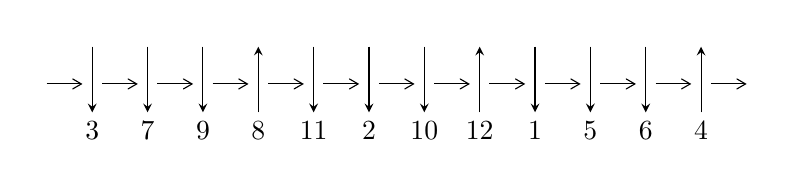
\begin{tikzpicture}[x=20pt, y=17pt]
	% nodes
	\node (C0) at (0, 0) {};
	\node (C1) at (1, 0) {};
	\node (C1U) at (1, +1) {};
	\node (C1D) at (1, -1) {3};

	\node (C2) at (2, 0) {};
	\node (C2U) at (2, +1) {};
	\node (C2D) at (2, -1) {7};

	\node (C3) at (3, 0) {};
	\node (C3U) at (3, +1) {};
	\node (C3D) at (3, -1) {9};

	\node (C4) at (4, 0) {};
	\node (C4U) at (4, +1) {};
	\node (C4D) at (4, -1) {8};

	\node (C5) at (5, 0) {};
	\node (C5U) at (5, +1) {};
	\node (C5D) at (5, -1) {11};

	\node (C6) at (6, 0) {};
	\node (C6U) at (6, +1) {};
	\node (C6D) at (6, -1) {2};

	\node (C7) at (7, 0) {};
	\node (C7U) at (7, +1) {};
	\node (C7D) at (7, -1) {10};

	\node (C8) at (8, 0) {};
	\node (C8U) at (8, +1) {};
	\node (C8D) at (8, -1) {12};

	\node (C9) at (9, 0) {};
	\node (C9U) at (9, +1) {};
	\node (C9D) at (9, -1) {1};

	\node (C10) at (10, 0) {};
	\node (C10U) at (10, +1) {};
	\node (C10D) at (10, -1) {5};

	\node (C11) at (11, 0) {};
	\node (C11U) at (11, +1) {};
	\node (C11D) at (11, -1) {6};

	\node (C12) at (12, 0) {};
	\node (C12U) at (12, +1) {};
	\node (C12D) at (12, -1) {4};
	\node (C13) at (13, 0) {};

	% arrows
	\draw[->,>={angle 60}]
	(C0) edge (C1) (C1) edge (C2) (C2) edge (C3) (C3) edge (C4) (C4) edge (C5) (C5) edge (C6) (C6) edge (C7) (C7) edge (C8) (C8) edge (C9) (C9) edge (C10) (C10) edge (C11) (C11) edge (C12) (C12) edge (C13) ;	\draw[->,>=stealth]
	(C1U) edge (C1D) (C2U) edge (C2D) (C3U) edge (C3D) (C4D) edge (C4U) (C5U) edge (C5D) (C6U) edge (C6D) (C7U) edge (C7D) (C8D) edge (C8U) (C9U) edge (C9D) (C10U) edge (C10D) (C11U) edge (C11D) (C12D) edge (C12U) ;
	\end{tikzpicture} \\
\hhline{~~} \\& 
\textbf{Solving Sequence} \\ \cline{2-2} 
 &
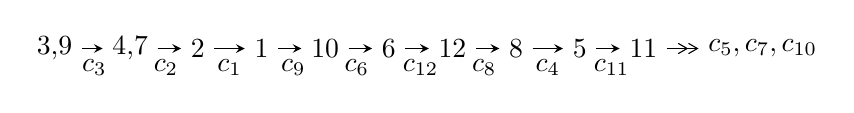
\begin{tikzpicture}[x=23pt, y=7pt]
	% node
	\node (A0) at (-1/8, 0) {3,9};
	\node (A1) at (17/16, 0) {4,7};
	\node (A2) at (17/8, 0) {2};
	\node (A3) at (25/8, 0) {1};
	\node (A4) at (33/8, 0) {10};
	\node (A5) at (41/8, 0) {6};
	\node (A6) at (49/8, 0) {12};
	\node (A7) at (57/8, 0) {8};
	\node (A8) at (65/8, 0) {5};
	\node (A9) at (73/8, 0) {11};
	\node (C1) at (1/2, -1) {$c_{3}$};
	\node (C2) at (13/8, -1) {$c_{2}$};
	\node (C3) at (21/8, -1) {$c_{1}$};
	\node (C4) at (29/8, -1) {$c_{9}$};
	\node (C5) at (37/8, -1) {$c_{6}$};
	\node (C6) at (45/8, -1) {$c_{12}$};
	\node (C7) at (53/8, -1) {$c_{8}$};
	\node (C8) at (61/8, -1) {$c_{4}$};
	\node (C9) at (69/8, -1) {$c_{11}$};
	\node (A10) at (11, 0) {$c_{5},c_{7},c_{10}$};

	% edge
	\draw[->,>=stealth]	
	(A0) edge (A1) (A1) edge (A2) (A2) edge (A3) (A3) edge (A4) (A4) edge (A5) (A5) edge (A6) (A6) edge (A7) (A7) edge (A8) (A8) edge (A9) ;
	\draw[->>,>={angle 60}]	
	(A9) edge (A10);
\end{tikzpicture} \\ 

\end{tabular} \\

\footnotetext{
The image of knot diagram is generated by the software ``\textbf{Draw programme}" developed by Andrew Bartholomew(\url{http://www.layer8.co.uk/maths/draw/index.htm\#Running-draw}), where we modified some parts for our purpose(\url{https://github.com/CATsTAILs/LinksPainter}).
}\phantom \\ \newline 
\centering \textbf{Ideals for irreducible components\footnotemark of $X_{\text{par}}$} 
 
\begin{align*}
I^u_{1}&=\langle 
1.96556\times10^{1272} u^{150}-4.61903\times10^{1272} u^{149}+\cdots+1.68074\times10^{1275} b-1.40593\times10^{1275},\\
\phantom{I^u_{1}}&\phantom{= \langle  }5.76019\times10^{1273} u^{150}+2.86320\times10^{1274} u^{149}+\cdots+7.54653\times10^{1277} a-2.77801\times10^{1278},\\
\phantom{I^u_{1}}&\phantom{= \langle  }u^{151}-2 u^{150}+\cdots+2162 u-449\rangle \\
I^u_{2}&=\langle 
-2.90007\times10^{40} u^{31}+3.42238\times10^{40} u^{30}+\cdots+1.17408\times10^{41} b+1.01177\times10^{41},\\
\phantom{I^u_{2}}&\phantom{= \langle  }3.04606\times10^{40} u^{31}-3.49551\times10^{40} u^{30}+\cdots+1.17408\times10^{41} a-9.77906\times10^{40},\;u^{32}- u^{31}+\cdots-3 u-1\rangle \\
I^u_{3}&=\langle 
u^2+b+u,\;- u^2+a- u+1,\;u^3+2 u^2+u+1\rangle \\
\\
\end{align*}
\raggedright * 3 irreducible components of $\dim_{\mathbb{C}}=0$, with total 186 representations.\\
\footnotetext{All coefficients of polynomials are rational numbers. But the coefficients are sometimes approximated in decimal forms when there is not enough margin.}
\newpage
\renewcommand{\arraystretch}{1}
\centering \section*{I. $I^u_{1}= \langle 1.97\times10^{1272} u^{150}-4.62\times10^{1272} u^{149}+\cdots+1.68\times10^{1275} b-1.41\times10^{1275},\;5.76\times10^{1273} u^{150}+2.86\times10^{1274} u^{149}+\cdots+7.55\times10^{1277} a-2.78\times10^{1278},\;u^{151}-2 u^{150}+\cdots+2162 u-449 \rangle$}
\flushleft \textbf{(i) Arc colorings}\\
\begin{tabular}{m{7pt} m{180pt} m{7pt} m{180pt} }
\flushright $a_{3}=$&$\begin{pmatrix}1\\0\end{pmatrix}$ \\
\flushright $a_{9}=$&$\begin{pmatrix}0\\u\end{pmatrix}$ \\
\flushright $a_{4}=$&$\begin{pmatrix}1\\u^2\end{pmatrix}$ \\
\flushright $a_{7}=$&$\begin{pmatrix}-0.0000763290 u^{150}-0.000379406 u^{149}+\cdots-31.9809 u+3.68117\\-0.00116946 u^{150}+0.00274821 u^{149}+\cdots+7.24694 u+0.836496\end{pmatrix}$ \\
\flushright $a_{2}=$&$\begin{pmatrix}-0.00168220 u^{150}+0.00590328 u^{149}+\cdots+65.0155 u-6.42701\\-6.64115\times10^{-6} u^{150}-0.000367296 u^{149}+\cdots-19.2980 u+0.0982350\end{pmatrix}$ \\
\flushright $a_{1}=$&$\begin{pmatrix}-0.00168885 u^{150}+0.00553599 u^{149}+\cdots+45.7175 u-6.32878\\-6.64115\times10^{-6} u^{150}-0.000367296 u^{149}+\cdots-19.2980 u+0.0982350\end{pmatrix}$ \\
\flushright $a_{10}=$&$\begin{pmatrix}0.0117674 u^{150}-0.0223322 u^{149}+\cdots+43.3172 u-11.8273\\-0.00133968 u^{150}+0.00299390 u^{149}+\cdots+2.76487 u+0.424849\end{pmatrix}$ \\
\flushright $a_{6}=$&$\begin{pmatrix}0.00568194 u^{150}-0.0122842 u^{149}+\cdots+31.1122 u-0.393206\\-0.00115135 u^{150}+0.00292564 u^{149}+\cdots-14.9915 u-1.56282\end{pmatrix}$ \\
\flushright $a_{12}=$&$\begin{pmatrix}-0.00168228 u^{150}+0.00557349 u^{149}+\cdots+59.5909 u-5.45794\\0.0000690792 u^{150}-0.000523140 u^{149}+\cdots-19.4045 u+0.120968\end{pmatrix}$ \\
\flushright $a_{8}=$&$\begin{pmatrix}0.0105884 u^{150}-0.0198923 u^{149}+\cdots+43.1103 u-12.0399\\-0.00148726 u^{150}+0.00330437 u^{149}+\cdots+4.10259 u+0.904460\end{pmatrix}$ \\
\flushright $a_{5}=$&$\begin{pmatrix}0.00860053 u^{150}-0.0223541 u^{149}+\cdots-59.6672 u+9.81945\\0.000393479 u^{150}-0.000364436 u^{149}+\cdots-2.69319 u-2.04299\end{pmatrix}$ \\
\flushright $a_{11}=$&$\begin{pmatrix}-0.00385075 u^{150}+0.0101935 u^{149}+\cdots+21.0110 u-8.58046\\0.000913499 u^{150}-0.00139895 u^{149}+\cdots+25.8880 u-0.0780800\end{pmatrix}$\\&\end{tabular}
\flushleft \textbf{(ii) Obstruction class $= -1$}\\~\\
\flushleft \textbf{(iii) Cusp Shapes $= 0.0168044 u^{150}-0.0359252 u^{149}+\cdots+562.956 u+69.1771$}\\~\\
\newpage\renewcommand{\arraystretch}{1}
\flushleft \textbf{(iv) u-Polynomials at the component}\newline \\
\begin{tabular}{m{50pt}|m{274pt}}
Crossings & \hspace{64pt}u-Polynomials at each crossing \\
\hline $$\begin{aligned}c_{1}\end{aligned}$$&$\begin{aligned}
&u^{151}+66 u^{150}+\cdots+185503 u+3481
\end{aligned}$\\
\hline $$\begin{aligned}c_{2},c_{6}\end{aligned}$$&$\begin{aligned}
&u^{151}-2 u^{150}+\cdots+255 u-59
\end{aligned}$\\
\hline $$\begin{aligned}c_{3}\end{aligned}$$&$\begin{aligned}
&u^{151}-2 u^{150}+\cdots+2162 u-449
\end{aligned}$\\
\hline $$\begin{aligned}c_{4}\end{aligned}$$&$\begin{aligned}
&u^{151}-6 u^{150}+\cdots-5051302 u-765269
\end{aligned}$\\
\hline $$\begin{aligned}c_{5},c_{10},c_{11}\end{aligned}$$&$\begin{aligned}
&u^{151}- u^{150}+\cdots+122 u+11
\end{aligned}$\\
\hline $$\begin{aligned}c_{7}\end{aligned}$$&$\begin{aligned}
&u^{151}+7 u^{150}+\cdots+2354104 u+756296
\end{aligned}$\\
\hline $$\begin{aligned}c_{8}\end{aligned}$$&$\begin{aligned}
&u^{151}+4 u^{150}+\cdots-5327 u+391
\end{aligned}$\\
\hline $$\begin{aligned}c_{9}\end{aligned}$$&$\begin{aligned}
&u^{151}+3 u^{150}+\cdots- u+1
\end{aligned}$\\
\hline $$\begin{aligned}c_{12}\end{aligned}$$&$\begin{aligned}
&u^{151}+14 u^{150}+\cdots+45 u+1
\end{aligned}$\\
\hline
\end{tabular}\\~\\
\newpage\renewcommand{\arraystretch}{1}
\flushleft \textbf{(v) Riley Polynomials at the component}\newline \\
\begin{tabular}{m{50pt}|m{274pt}}
Crossings & \hspace{64pt}Riley Polynomials at each crossing \\
\hline $$\begin{aligned}c_{1}\end{aligned}$$&$\begin{aligned}
&y^{151}+42 y^{150}+\cdots-823270257 y-12117361
\end{aligned}$\\
\hline $$\begin{aligned}c_{2},c_{6}\end{aligned}$$&$\begin{aligned}
&y^{151}-66 y^{150}+\cdots+185503 y-3481
\end{aligned}$\\
\hline $$\begin{aligned}c_{3}\end{aligned}$$&$\begin{aligned}
&y^{151}+22 y^{150}+\cdots+18108324 y-201601
\end{aligned}$\\
\hline $$\begin{aligned}c_{4}\end{aligned}$$&$\begin{aligned}
&y^{151}+42 y^{150}+\cdots-16103090955074 y-585636642361
\end{aligned}$\\
\hline $$\begin{aligned}c_{5},c_{10},c_{11}\end{aligned}$$&$\begin{aligned}
&y^{151}-147 y^{150}+\cdots+43638 y-121
\end{aligned}$\\
\hline $$\begin{aligned}c_{7}\end{aligned}$$&$\begin{aligned}
&y^{151}-35 y^{150}+\cdots+10638457160160 y-571983639616
\end{aligned}$\\
\hline $$\begin{aligned}c_{8}\end{aligned}$$&$\begin{aligned}
&y^{151}+6 y^{150}+\cdots-424913 y-152881
\end{aligned}$\\
\hline $$\begin{aligned}c_{9}\end{aligned}$$&$\begin{aligned}
&y^{151}+17 y^{150}+\cdots+133 y-1
\end{aligned}$\\
\hline $$\begin{aligned}c_{12}\end{aligned}$$&$\begin{aligned}
&y^{151}+6 y^{150}+\cdots+293 y-1
\end{aligned}$\\
\hline
\end{tabular}\\~\\
\newpage\flushleft \textbf{(vi) Complex Volumes and Cusp Shapes}
$$\begin{array}{c|c|c}  
\text{Solutions to }I^u_{1}& \I (\text{vol} + \sqrt{-1}CS) & \text{Cusp shape}\\
 \hline 
\begin{aligned}
u &= -0.039981 + 1.008940 I \\
a &= -0.563623 + 1.213530 I \\
b &= \phantom{-}0.801162 - 0.706079 I\end{aligned}
 & \phantom{-}2.47108 + 2.65288 I & \phantom{-0.000000 } 0 \\ \hline\begin{aligned}
u &= -0.039981 - 1.008940 I \\
a &= -0.563623 - 1.213530 I \\
b &= \phantom{-}0.801162 + 0.706079 I\end{aligned}
 & \phantom{-}2.47108 - 2.65288 I & \phantom{-0.000000 } 0 \\ \hline\begin{aligned}
u &= \phantom{-}0.703513 + 0.695907 I \\
a &= -0.618455 + 0.040468 I \\
b &= -1.177490 + 0.116883 I\end{aligned}
 & -4.41545 - 2.22036 I & \phantom{-0.000000 } 0 \\ \hline\begin{aligned}
u &= \phantom{-}0.703513 - 0.695907 I \\
a &= -0.618455 - 0.040468 I \\
b &= -1.177490 - 0.116883 I\end{aligned}
 & -4.41545 + 2.22036 I & \phantom{-0.000000 } 0 \\ \hline\begin{aligned}
u &= \phantom{-}0.939145 + 0.409369 I \\
a &= \phantom{-}0.0896863 + 0.0368558 I \\
b &= \phantom{-}0.515699 - 0.698015 I\end{aligned}
 & -6.34616 - 4.01409 I & \phantom{-0.000000 } 0 \\ \hline\begin{aligned}
u &= \phantom{-}0.939145 - 0.409369 I \\
a &= \phantom{-}0.0896863 - 0.0368558 I \\
b &= \phantom{-}0.515699 + 0.698015 I\end{aligned}
 & -6.34616 + 4.01409 I & \phantom{-0.000000 } 0 \\ \hline\begin{aligned}
u &= \phantom{-}0.713828 + 0.650377 I \\
a &= -0.98542 + 2.10443 I \\
b &= -0.970801 - 0.659759 I\end{aligned}
 & -0.55710 - 6.66250 I & \phantom{-0.000000 } 0 \\ \hline\begin{aligned}
u &= \phantom{-}0.713828 - 0.650377 I \\
a &= -0.98542 - 2.10443 I \\
b &= -0.970801 + 0.659759 I\end{aligned}
 & -0.55710 + 6.66250 I & \phantom{-0.000000 } 0 \\ \hline\begin{aligned}
u &= -0.537746 + 0.891491 I \\
a &= \phantom{-}0.287736 + 1.187750 I \\
b &= -0.847487 - 0.680236 I\end{aligned}
 & -1.241290 + 0.238635 I & \phantom{-0.000000 } 0 \\ \hline\begin{aligned}
u &= -0.537746 - 0.891491 I \\
a &= \phantom{-}0.287736 - 1.187750 I \\
b &= -0.847487 + 0.680236 I\end{aligned}
 & -1.241290 - 0.238635 I & \phantom{-0.000000 } 0\\
 \hline 
 \end{array}$$\newpage$$\begin{array}{c|c|c}  
\text{Solutions to }I^u_{1}& \I (\text{vol} + \sqrt{-1}CS) & \text{Cusp shape}\\
 \hline 
\begin{aligned}
u &= \phantom{-}1.001240 + 0.291819 I \\
a &= \phantom{-}0.195006 - 1.234500 I \\
b &= \phantom{-}0.305382 + 0.450804 I\end{aligned}
 & -0.31238 + 2.57038 I & \phantom{-0.000000 } 0 \\ \hline\begin{aligned}
u &= \phantom{-}1.001240 - 0.291819 I \\
a &= \phantom{-}0.195006 + 1.234500 I \\
b &= \phantom{-}0.305382 - 0.450804 I\end{aligned}
 & -0.31238 - 2.57038 I & \phantom{-0.000000 } 0 \\ \hline\begin{aligned}
u &= \phantom{-}0.884487 + 0.346998 I \\
a &= -0.187209 - 0.686003 I \\
b &= \phantom{-}1.335700 + 0.443505 I\end{aligned}
 & -8.59510 + 0.02221 I & \phantom{-0.000000 } 0 \\ \hline\begin{aligned}
u &= \phantom{-}0.884487 - 0.346998 I \\
a &= -0.187209 + 0.686003 I \\
b &= \phantom{-}1.335700 - 0.443505 I\end{aligned}
 & -8.59510 - 0.02221 I & \phantom{-0.000000 } 0 \\ \hline\begin{aligned}
u &= \phantom{-}0.656850 + 0.850604 I \\
a &= \phantom{-}0.921131 - 0.469165 I \\
b &= \phantom{-}0.359459 + 0.262040 I\end{aligned}
 & -6.51533 - 2.97279 I & \phantom{-0.000000 } 0 \\ \hline\begin{aligned}
u &= \phantom{-}0.656850 - 0.850604 I \\
a &= \phantom{-}0.921131 + 0.469165 I \\
b &= \phantom{-}0.359459 - 0.262040 I\end{aligned}
 & -6.51533 + 2.97279 I & \phantom{-0.000000 } 0 \\ \hline\begin{aligned}
u &= \phantom{-}0.740056 + 0.783206 I \\
a &= \phantom{-}0.133832 - 0.599426 I \\
b &= -0.138405 + 0.827201 I\end{aligned}
 & -6.77489 - 2.11958 I & \phantom{-0.000000 } 0 \\ \hline\begin{aligned}
u &= \phantom{-}0.740056 - 0.783206 I \\
a &= \phantom{-}0.133832 + 0.599426 I \\
b &= -0.138405 - 0.827201 I\end{aligned}
 & -6.77489 + 2.11958 I & \phantom{-0.000000 } 0 \\ \hline\begin{aligned}
u &= \phantom{-}0.684530 + 0.845794 I \\
a &= \phantom{-}0.851637 + 0.866097 I \\
b &= -0.911724 + 0.255229 I\end{aligned}
 & -7.33520 - 4.69044 I & \phantom{-0.000000 } 0 \\ \hline\begin{aligned}
u &= \phantom{-}0.684530 - 0.845794 I \\
a &= \phantom{-}0.851637 - 0.866097 I \\
b &= -0.911724 - 0.255229 I\end{aligned}
 & -7.33520 + 4.69044 I & \phantom{-0.000000 } 0\\
 \hline 
 \end{array}$$\newpage$$\begin{array}{c|c|c}  
\text{Solutions to }I^u_{1}& \I (\text{vol} + \sqrt{-1}CS) & \text{Cusp shape}\\
 \hline 
\begin{aligned}
u &= -0.874553 + 0.236922 I \\
a &= -0.063913 + 0.716291 I \\
b &= -0.998554 - 0.380216 I\end{aligned}
 & -1.65732 - 0.38865 I & \phantom{-0.000000 } 0 \\ \hline\begin{aligned}
u &= -0.874553 - 0.236922 I \\
a &= -0.063913 - 0.716291 I \\
b &= -0.998554 + 0.380216 I\end{aligned}
 & -1.65732 + 0.38865 I & \phantom{-0.000000 } 0 \\ \hline\begin{aligned}
u &= -0.414158 + 0.803206 I \\
a &= -0.19220 - 1.61244 I \\
b &= -1.184650 + 0.708377 I\end{aligned}
 & -4.67562 + 11.48670 I & \phantom{-0.000000 } 0 \\ \hline\begin{aligned}
u &= -0.414158 - 0.803206 I \\
a &= -0.19220 + 1.61244 I \\
b &= -1.184650 - 0.708377 I\end{aligned}
 & -4.67562 - 11.48670 I & \phantom{-0.000000 } 0 \\ \hline\begin{aligned}
u &= -0.633732 + 0.638046 I \\
a &= \phantom{-}1.054430 + 0.057142 I \\
b &= -0.679572 - 0.679532 I\end{aligned}
 & \phantom{-}0.30481 + 1.46754 I & \phantom{-0.000000 } 0 \\ \hline\begin{aligned}
u &= -0.633732 - 0.638046 I \\
a &= \phantom{-}1.054430 - 0.057142 I \\
b &= -0.679572 + 0.679532 I\end{aligned}
 & \phantom{-}0.30481 - 1.46754 I & \phantom{-0.000000 } 0 \\ \hline\begin{aligned}
u &= -1.065660 + 0.299057 I \\
a &= \phantom{-}1.027770 + 0.819795 I \\
b &= \phantom{-}1.047810 - 0.626072 I\end{aligned}
 & -7.88222 + 9.14328 I & \phantom{-0.000000 } 0 \\ \hline\begin{aligned}
u &= -1.065660 - 0.299057 I \\
a &= \phantom{-}1.027770 - 0.819795 I \\
b &= \phantom{-}1.047810 + 0.626072 I\end{aligned}
 & -7.88222 - 9.14328 I & \phantom{-0.000000 } 0 \\ \hline\begin{aligned}
u &= -0.054378 + 0.887305 I \\
a &= \phantom{-}0.657565 + 0.023569 I \\
b &= -0.475200 + 0.545615 I\end{aligned}
 & \phantom{-}1.95450 + 3.17739 I & \phantom{-0.000000 } 0 \\ \hline\begin{aligned}
u &= -0.054378 - 0.887305 I \\
a &= \phantom{-}0.657565 - 0.023569 I \\
b &= -0.475200 - 0.545615 I\end{aligned}
 & \phantom{-}1.95450 - 3.17739 I & \phantom{-0.000000 } 0\\
 \hline 
 \end{array}$$\newpage$$\begin{array}{c|c|c}  
\text{Solutions to }I^u_{1}& \I (\text{vol} + \sqrt{-1}CS) & \text{Cusp shape}\\
 \hline 
\begin{aligned}
u &= -0.486191 + 1.013690 I \\
a &= -0.358459 + 0.571467 I \\
b &= \phantom{-}0.270776 - 0.096317 I\end{aligned}
 & \phantom{-}0.87014 + 3.15700 I & \phantom{-0.000000 } 0 \\ \hline\begin{aligned}
u &= -0.486191 - 1.013690 I \\
a &= -0.358459 - 0.571467 I \\
b &= \phantom{-}0.270776 + 0.096317 I\end{aligned}
 & \phantom{-}0.87014 - 3.15700 I & \phantom{-0.000000 } 0 \\ \hline\begin{aligned}
u &= -0.349386 + 0.779593 I \\
a &= -1.93148 + 0.79619 I \\
b &= \phantom{-}0.824113 + 0.461791 I\end{aligned}
 & \phantom{-}0.75907 + 1.21132 I & \phantom{-0.000000 } 0 \\ \hline\begin{aligned}
u &= -0.349386 - 0.779593 I \\
a &= -1.93148 - 0.79619 I \\
b &= \phantom{-}0.824113 - 0.461791 I\end{aligned}
 & \phantom{-}0.75907 - 1.21132 I & \phantom{-0.000000 } 0 \\ \hline\begin{aligned}
u &= \phantom{-}0.510108 + 0.682296 I \\
a &= \phantom{-}0.332547 + 1.273250 I \\
b &= -0.402137 - 0.983875 I\end{aligned}
 & \phantom{-}1.43305 - 4.63133 I & \phantom{-0.000000 } 0 \\ \hline\begin{aligned}
u &= \phantom{-}0.510108 - 0.682296 I \\
a &= \phantom{-}0.332547 - 1.273250 I \\
b &= -0.402137 + 0.983875 I\end{aligned}
 & \phantom{-}1.43305 + 4.63133 I & \phantom{-0.000000 } 0 \\ \hline\begin{aligned}
u &= -0.170544 + 0.821873 I \\
a &= -0.45307 + 1.94856 I \\
b &= \phantom{-}0.864012 - 0.660336 I\end{aligned}
 & \phantom{-}2.31706 + 2.60082 I & \phantom{-0.000000 } 0 \\ \hline\begin{aligned}
u &= -0.170544 - 0.821873 I \\
a &= -0.45307 - 1.94856 I \\
b &= \phantom{-}0.864012 + 0.660336 I\end{aligned}
 & \phantom{-}2.31706 - 2.60082 I & \phantom{-0.000000 } 0 \\ \hline\begin{aligned}
u &= \phantom{-}1.172680 + 0.270553 I \\
a &= \phantom{-}0.561705 + 1.044390 I \\
b &= \phantom{-}0.692677 - 0.246807 I\end{aligned}
 & -0.34895 - 2.72408 I & \phantom{-0.000000 } 0 \\ \hline\begin{aligned}
u &= \phantom{-}1.172680 - 0.270553 I \\
a &= \phantom{-}0.561705 - 1.044390 I \\
b &= \phantom{-}0.692677 + 0.246807 I\end{aligned}
 & -0.34895 + 2.72408 I & \phantom{-0.000000 } 0\\
 \hline 
 \end{array}$$\newpage$$\begin{array}{c|c|c}  
\text{Solutions to }I^u_{1}& \I (\text{vol} + \sqrt{-1}CS) & \text{Cusp shape}\\
 \hline 
\begin{aligned}
u &= -1.20530\phantom{ +0.000000I} \\
a &= \phantom{-}0.119339\phantom{ +0.000000I} \\
b &= -1.28443\phantom{ +0.000000I}\end{aligned}
 & -2.37234\phantom{ +0.000000I} & \phantom{-0.000000 } 0 \\ \hline\begin{aligned}
u &= -0.035138 + 0.791480 I \\
a &= -0.688063 - 0.627838 I \\
b &= \phantom{-}0.434675 + 0.841979 I\end{aligned}
 & \phantom{-}3.61412 + 1.43650 I & \phantom{-0.000000 } 0 \\ \hline\begin{aligned}
u &= -0.035138 - 0.791480 I \\
a &= -0.688063 + 0.627838 I \\
b &= \phantom{-}0.434675 - 0.841979 I\end{aligned}
 & \phantom{-}3.61412 - 1.43650 I & \phantom{-0.000000 } 0 \\ \hline\begin{aligned}
u &= \phantom{-}0.707109 + 0.352643 I \\
a &= \phantom{-}1.69700 - 0.31512 I \\
b &= \phantom{-}0.980235 + 0.009187 I\end{aligned}
 & -4.60050 - 1.41999 I & \phantom{-0.000000 } 0 \\ \hline\begin{aligned}
u &= \phantom{-}0.707109 - 0.352643 I \\
a &= \phantom{-}1.69700 + 0.31512 I \\
b &= \phantom{-}0.980235 - 0.009187 I\end{aligned}
 & -4.60050 + 1.41999 I & \phantom{-0.000000 } 0 \\ \hline\begin{aligned}
u &= \phantom{-}0.343900 + 0.703421 I \\
a &= \phantom{-}0.54662 - 1.51724 I \\
b &= \phantom{-}1.139670 + 0.641881 I\end{aligned}
 & \phantom{-}1.48391 - 6.97874 I & \phantom{-0.000000 } 0 \\ \hline\begin{aligned}
u &= \phantom{-}0.343900 - 0.703421 I \\
a &= \phantom{-}0.54662 + 1.51724 I \\
b &= \phantom{-}1.139670 - 0.641881 I\end{aligned}
 & \phantom{-}1.48391 + 6.97874 I & \phantom{-0.000000 } 0 \\ \hline\begin{aligned}
u &= -0.684542 + 0.375884 I \\
a &= \phantom{-}0.565949 - 0.523686 I \\
b &= \phantom{-}1.273910 + 0.251148 I\end{aligned}
 & -11.42070 - 1.71813 I & \phantom{-0.000000 } 0 \\ \hline\begin{aligned}
u &= -0.684542 - 0.375884 I \\
a &= \phantom{-}0.565949 + 0.523686 I \\
b &= \phantom{-}1.273910 - 0.251148 I\end{aligned}
 & -11.42070 + 1.71813 I & \phantom{-0.000000 } 0 \\ \hline\begin{aligned}
u &= -0.774735 + 0.028512 I \\
a &= -1.39398 + 1.10712 I \\
b &= -1.115300 - 0.091313 I\end{aligned}
 & -11.30190 + 2.36606 I & \phantom{-0.000000 } 0\\
 \hline 
 \end{array}$$\newpage$$\begin{array}{c|c|c}  
\text{Solutions to }I^u_{1}& \I (\text{vol} + \sqrt{-1}CS) & \text{Cusp shape}\\
 \hline 
\begin{aligned}
u &= -0.774735 - 0.028512 I \\
a &= -1.39398 - 1.10712 I \\
b &= -1.115300 + 0.091313 I\end{aligned}
 & -11.30190 - 2.36606 I & \phantom{-0.000000 } 0 \\ \hline\begin{aligned}
u &= \phantom{-}0.971948 + 0.754721 I \\
a &= -0.279676 - 0.490526 I \\
b &= -0.934466 + 0.481120 I\end{aligned}
 & -2.16344 + 2.84576 I & \phantom{-0.000000 } 0 \\ \hline\begin{aligned}
u &= \phantom{-}0.971948 - 0.754721 I \\
a &= -0.279676 + 0.490526 I \\
b &= -0.934466 - 0.481120 I\end{aligned}
 & -2.16344 - 2.84576 I & \phantom{-0.000000 } 0 \\ \hline\begin{aligned}
u &= -0.019191 + 0.758227 I \\
a &= -1.42992 + 2.58015 I \\
b &= \phantom{-}0.840519 - 0.669274 I\end{aligned}
 & \phantom{-}2.17960 + 2.59133 I & \phantom{-0.000000 } 0 \\ \hline\begin{aligned}
u &= -0.019191 - 0.758227 I \\
a &= -1.42992 - 2.58015 I \\
b &= \phantom{-}0.840519 + 0.669274 I\end{aligned}
 & \phantom{-}2.17960 - 2.59133 I & \phantom{-0.000000 } 0 \\ \hline\begin{aligned}
u &= \phantom{-}0.799867 + 0.949650 I \\
a &= \phantom{-}0.14204 + 1.58333 I \\
b &= -0.925437 - 0.691493 I\end{aligned}
 & -1.57764 - 5.52140 I & \phantom{-0.000000 } 0 \\ \hline\begin{aligned}
u &= \phantom{-}0.799867 - 0.949650 I \\
a &= \phantom{-}0.14204 - 1.58333 I \\
b &= -0.925437 + 0.691493 I\end{aligned}
 & -1.57764 + 5.52140 I & \phantom{-0.000000 } 0 \\ \hline\begin{aligned}
u &= -0.927660 + 0.825764 I \\
a &= \phantom{-}0.300167 + 0.279865 I \\
b &= \phantom{-}1.231230 - 0.033904 I\end{aligned}
 & -4.71028 + 7.33856 I & \phantom{-0.000000 } 0 \\ \hline\begin{aligned}
u &= -0.927660 - 0.825764 I \\
a &= \phantom{-}0.300167 - 0.279865 I \\
b &= \phantom{-}1.231230 + 0.033904 I\end{aligned}
 & -4.71028 - 7.33856 I & \phantom{-0.000000 } 0 \\ \hline\begin{aligned}
u &= \phantom{-}0.116359 + 0.748309 I \\
a &= \phantom{-}0.625750 - 0.998270 I \\
b &= -0.425643 + 1.056950 I\end{aligned}
 & -2.34326 - 5.17950 I & \phantom{-0.000000 } 0\\
 \hline 
 \end{array}$$\newpage$$\begin{array}{c|c|c}  
\text{Solutions to }I^u_{1}& \I (\text{vol} + \sqrt{-1}CS) & \text{Cusp shape}\\
 \hline 
\begin{aligned}
u &= \phantom{-}0.116359 - 0.748309 I \\
a &= \phantom{-}0.625750 + 0.998270 I \\
b &= -0.425643 - 1.056950 I\end{aligned}
 & -2.34326 + 5.17950 I & \phantom{-0.000000 } 0 \\ \hline\begin{aligned}
u &= \phantom{-}0.479187 + 0.567765 I \\
a &= \phantom{-}2.15146 - 1.72457 I \\
b &= \phantom{-}0.928810 + 0.502544 I\end{aligned}
 & \phantom{-}0.34784 - 5.12983 I & \phantom{-0.000000 } 0 \\ \hline\begin{aligned}
u &= \phantom{-}0.479187 - 0.567765 I \\
a &= \phantom{-}2.15146 + 1.72457 I \\
b &= \phantom{-}0.928810 - 0.502544 I\end{aligned}
 & \phantom{-}0.34784 + 5.12983 I & \phantom{-0.000000 } 0 \\ \hline\begin{aligned}
u &= -0.973470 + 0.807792 I \\
a &= -0.650484 - 1.157520 I \\
b &= -1.129410 + 0.509755 I\end{aligned}
 & -9.68944 + 6.79778 I & \phantom{-0.000000 } 0 \\ \hline\begin{aligned}
u &= -0.973470 - 0.807792 I \\
a &= -0.650484 + 1.157520 I \\
b &= -1.129410 - 0.509755 I\end{aligned}
 & -9.68944 - 6.79778 I & \phantom{-0.000000 } 0 \\ \hline\begin{aligned}
u &= -0.588303 + 0.421762 I \\
a &= -0.38630 + 1.47599 I \\
b &= \phantom{-}0.444568 - 1.254430 I\end{aligned}
 & -4.56487 + 6.76711 I & \phantom{-0.000000 } 0 \\ \hline\begin{aligned}
u &= -0.588303 - 0.421762 I \\
a &= -0.38630 - 1.47599 I \\
b &= \phantom{-}0.444568 + 1.254430 I\end{aligned}
 & -4.56487 - 6.76711 I & \phantom{-0.000000 } 0 \\ \hline\begin{aligned}
u &= -0.548054 + 0.469018 I \\
a &= -0.272258 - 0.565473 I \\
b &= -0.321105 + 0.348772 I\end{aligned}
 & -0.981069 + 0.675049 I & \phantom{-0.000000 } 0 \\ \hline\begin{aligned}
u &= -0.548054 - 0.469018 I \\
a &= -0.272258 + 0.565473 I \\
b &= -0.321105 - 0.348772 I\end{aligned}
 & -0.981069 - 0.675049 I & \phantom{-0.000000 } 0 \\ \hline\begin{aligned}
u &= -0.699564 + 1.080760 I \\
a &= -0.684863 - 0.689021 I \\
b &= \phantom{-}0.463445 + 0.766465 I\end{aligned}
 & \phantom{-}0.81996 + 4.40543 I & \phantom{-0.000000 } 0\\
 \hline 
 \end{array}$$\newpage$$\begin{array}{c|c|c}  
\text{Solutions to }I^u_{1}& \I (\text{vol} + \sqrt{-1}CS) & \text{Cusp shape}\\
 \hline 
\begin{aligned}
u &= -0.699564 - 1.080760 I \\
a &= -0.684863 + 0.689021 I \\
b &= \phantom{-}0.463445 - 0.766465 I\end{aligned}
 & \phantom{-}0.81996 - 4.40543 I & \phantom{-0.000000 } 0 \\ \hline\begin{aligned}
u &= \phantom{-}0.264880 + 1.265290 I \\
a &= \phantom{-}0.774566 + 1.042540 I \\
b &= -0.893724 - 0.530535 I\end{aligned}
 & -1.61994 - 4.80324 I & \phantom{-0.000000 } 0 \\ \hline\begin{aligned}
u &= \phantom{-}0.264880 - 1.265290 I \\
a &= \phantom{-}0.774566 - 1.042540 I \\
b &= -0.893724 + 0.530535 I\end{aligned}
 & -1.61994 + 4.80324 I & \phantom{-0.000000 } 0 \\ \hline\begin{aligned}
u &= \phantom{-}0.103422 + 0.685721 I \\
a &= \phantom{-}3.05287 + 0.04453 I \\
b &= -0.886886 + 0.550508 I\end{aligned}
 & \phantom{-}1.47781 + 5.10675 I & \phantom{-0.000000 } 0 \\ \hline\begin{aligned}
u &= \phantom{-}0.103422 - 0.685721 I \\
a &= \phantom{-}3.05287 - 0.04453 I \\
b &= -0.886886 - 0.550508 I\end{aligned}
 & \phantom{-}1.47781 - 5.10675 I & \phantom{-0.000000 } 0 \\ \hline\begin{aligned}
u &= -0.024085 + 1.310030 I \\
a &= \phantom{-}0.29059 - 2.09296 I \\
b &= -0.690944 + 0.464454 I\end{aligned}
 & -6.34572 - 1.76164 I & \phantom{-0.000000 } 0 \\ \hline\begin{aligned}
u &= -0.024085 - 1.310030 I \\
a &= \phantom{-}0.29059 + 2.09296 I \\
b &= -0.690944 - 0.464454 I\end{aligned}
 & -6.34572 + 1.76164 I & \phantom{-0.000000 } 0 \\ \hline\begin{aligned}
u &= -0.329046 + 0.599417 I \\
a &= \phantom{-}0.62690 + 1.89085 I \\
b &= -0.709570 - 0.545400 I\end{aligned}
 & -1.210210 + 0.420943 I & \phantom{-0.000000 } 0 \\ \hline\begin{aligned}
u &= -0.329046 - 0.599417 I \\
a &= \phantom{-}0.62690 - 1.89085 I \\
b &= -0.709570 + 0.545400 I\end{aligned}
 & -1.210210 - 0.420943 I & \phantom{-0.000000 } 0 \\ \hline\begin{aligned}
u &= \phantom{-}1.32170\phantom{ +0.000000I} \\
a &= -0.458239\phantom{ +0.000000I} \\
b &= \phantom{-}1.49086\phantom{ +0.000000I}\end{aligned}
 & -6.91048\phantom{ +0.000000I} & \phantom{-0.000000 } 0\\
 \hline 
 \end{array}$$\newpage$$\begin{array}{c|c|c}  
\text{Solutions to }I^u_{1}& \I (\text{vol} + \sqrt{-1}CS) & \text{Cusp shape}\\
 \hline 
\begin{aligned}
u &= \phantom{-}0.089553 + 0.661013 I \\
a &= -3.10919 - 1.51787 I \\
b &= \phantom{-}0.976704 + 0.580862 I\end{aligned}
 & -5.28622 - 9.93901 I & \phantom{-0.000000 } 0 \\ \hline\begin{aligned}
u &= \phantom{-}0.089553 - 0.661013 I \\
a &= -3.10919 + 1.51787 I \\
b &= \phantom{-}0.976704 - 0.580862 I\end{aligned}
 & -5.28622 + 9.93901 I & \phantom{-0.000000 } 0 \\ \hline\begin{aligned}
u &= -0.841993 + 1.037930 I \\
a &= \phantom{-}0.246589 + 1.260550 I \\
b &= -0.276920 - 0.999554 I\end{aligned}
 & -0.18904 + 4.43856 I & \phantom{-0.000000 } 0 \\ \hline\begin{aligned}
u &= -0.841993 - 1.037930 I \\
a &= \phantom{-}0.246589 - 1.260550 I \\
b &= -0.276920 + 0.999554 I\end{aligned}
 & -0.18904 - 4.43856 I & \phantom{-0.000000 } 0 \\ \hline\begin{aligned}
u &= -1.234190 + 0.517934 I \\
a &= -0.32568 - 1.46809 I \\
b &= -0.204742 + 0.521959 I\end{aligned}
 & -5.87844 - 5.67462 I & \phantom{-0.000000 } 0 \\ \hline\begin{aligned}
u &= -1.234190 - 0.517934 I \\
a &= -0.32568 + 1.46809 I \\
b &= -0.204742 - 0.521959 I\end{aligned}
 & -5.87844 + 5.67462 I & \phantom{-0.000000 } 0 \\ \hline\begin{aligned}
u &= -1.336730 + 0.092485 I \\
a &= -0.88139 + 1.24930 I \\
b &= -0.520147 - 0.180317 I\end{aligned}
 & -5.84098 + 5.80109 I & \phantom{-0.000000 } 0 \\ \hline\begin{aligned}
u &= -1.336730 - 0.092485 I \\
a &= -0.88139 - 1.24930 I \\
b &= -0.520147 + 0.180317 I\end{aligned}
 & -5.84098 - 5.80109 I & \phantom{-0.000000 } 0 \\ \hline\begin{aligned}
u &= \phantom{-}1.110730 + 0.781094 I \\
a &= -0.022663 + 0.254977 I \\
b &= -1.350050 - 0.077479 I\end{aligned}
 & -11.5645 - 10.7900 I & \phantom{-0.000000 } 0 \\ \hline\begin{aligned}
u &= \phantom{-}1.110730 - 0.781094 I \\
a &= -0.022663 - 0.254977 I \\
b &= -1.350050 + 0.077479 I\end{aligned}
 & -11.5645 + 10.7900 I & \phantom{-0.000000 } 0\\
 \hline 
 \end{array}$$\newpage$$\begin{array}{c|c|c}  
\text{Solutions to }I^u_{1}& \I (\text{vol} + \sqrt{-1}CS) & \text{Cusp shape}\\
 \hline 
\begin{aligned}
u &= -0.647621 + 1.201000 I \\
a &= \phantom{-}0.762783 + 1.103760 I \\
b &= -0.705171 - 0.872448 I\end{aligned}
 & \phantom{-}0.385022 + 0.107964 I & \phantom{-0.000000 } 0 \\ \hline\begin{aligned}
u &= -0.647621 - 1.201000 I \\
a &= \phantom{-}0.762783 - 1.103760 I \\
b &= -0.705171 + 0.872448 I\end{aligned}
 & \phantom{-}0.385022 - 0.107964 I & \phantom{-0.000000 } 0 \\ \hline\begin{aligned}
u &= \phantom{-}0.769908 + 1.153220 I \\
a &= -0.472047 + 1.079770 I \\
b &= \phantom{-}0.509078 - 0.857408 I\end{aligned}
 & \phantom{-}3.87805 - 2.26852 I & \phantom{-0.000000 } 0 \\ \hline\begin{aligned}
u &= \phantom{-}0.769908 - 1.153220 I \\
a &= -0.472047 - 1.079770 I \\
b &= \phantom{-}0.509078 + 0.857408 I\end{aligned}
 & \phantom{-}3.87805 + 2.26852 I & \phantom{-0.000000 } 0 \\ \hline\begin{aligned}
u &= \phantom{-}0.698278 + 1.201230 I \\
a &= -0.02692 + 1.90099 I \\
b &= -0.998175 - 0.747753 I\end{aligned}
 & -0.52356 - 6.09369 I & \phantom{-0.000000 } 0 \\ \hline\begin{aligned}
u &= \phantom{-}0.698278 - 1.201230 I \\
a &= -0.02692 - 1.90099 I \\
b &= -0.998175 + 0.747753 I\end{aligned}
 & -0.52356 + 6.09369 I & \phantom{-0.000000 } 0 \\ \hline\begin{aligned}
u &= -0.251881 + 0.531550 I \\
a &= -0.938753 - 0.899272 I \\
b &= -1.141050 + 0.529975 I\end{aligned}
 & -0.120299 + 1.210570 I & -9.4715 - 13.8749 I \\ \hline\begin{aligned}
u &= -0.251881 - 0.531550 I \\
a &= -0.938753 + 0.899272 I \\
b &= -1.141050 - 0.529975 I\end{aligned}
 & -0.120299 - 1.210570 I & -9.4715 + 13.8749 I \\ \hline\begin{aligned}
u &= \phantom{-}0.87395 + 1.11199 I \\
a &= \phantom{-}0.39038 - 1.65013 I \\
b &= \phantom{-}1.086800 + 0.627696 I\end{aligned}
 & -1.00826 - 9.69803 I & \phantom{-0.000000 } 0 \\ \hline\begin{aligned}
u &= \phantom{-}0.87395 - 1.11199 I \\
a &= \phantom{-}0.39038 + 1.65013 I \\
b &= \phantom{-}1.086800 - 0.627696 I\end{aligned}
 & -1.00826 + 9.69803 I & \phantom{-0.000000 } 0\\
 \hline 
 \end{array}$$\newpage$$\begin{array}{c|c|c}  
\text{Solutions to }I^u_{1}& \I (\text{vol} + \sqrt{-1}CS) & \text{Cusp shape}\\
 \hline 
\begin{aligned}
u &= \phantom{-}0.83764 + 1.17107 I \\
a &= \phantom{-}0.652409 - 0.941387 I \\
b &= -0.515383 + 0.903941 I\end{aligned}
 & \phantom{-}1.90280 - 9.41620 I & \phantom{-0.000000 } 0 \\ \hline\begin{aligned}
u &= \phantom{-}0.83764 - 1.17107 I \\
a &= \phantom{-}0.652409 + 0.941387 I \\
b &= -0.515383 - 0.903941 I\end{aligned}
 & \phantom{-}1.90280 + 9.41620 I & \phantom{-0.000000 } 0 \\ \hline\begin{aligned}
u &= \phantom{-}0.26966 + 1.44054 I \\
a &= -0.37076 - 1.73682 I \\
b &= \phantom{-}0.882042 + 0.460269 I\end{aligned}
 & -2.53359 - 1.87365 I & \phantom{-0.000000 } 0 \\ \hline\begin{aligned}
u &= \phantom{-}0.26966 - 1.44054 I \\
a &= -0.37076 + 1.73682 I \\
b &= \phantom{-}0.882042 - 0.460269 I\end{aligned}
 & -2.53359 + 1.87365 I & \phantom{-0.000000 } 0 \\ \hline\begin{aligned}
u &= -0.233905 + 0.464300 I \\
a &= -0.58755 + 2.61761 I \\
b &= \phantom{-}1.099530 - 0.808893 I\end{aligned}
 & -5.22555 + 4.13773 I & -14.9345 - 2.8334 I \\ \hline\begin{aligned}
u &= -0.233905 - 0.464300 I \\
a &= -0.58755 - 2.61761 I \\
b &= \phantom{-}1.099530 + 0.808893 I\end{aligned}
 & -5.22555 - 4.13773 I & -14.9345 + 2.8334 I \\ \hline\begin{aligned}
u &= -0.94984 + 1.18248 I \\
a &= -0.587432 - 1.051910 I \\
b &= \phantom{-}0.514050 + 0.989899 I\end{aligned}
 & -4.18881 + 13.48630 I & \phantom{-0.000000 } 0 \\ \hline\begin{aligned}
u &= -0.94984 - 1.18248 I \\
a &= -0.587432 + 1.051910 I \\
b &= \phantom{-}0.514050 - 0.989899 I\end{aligned}
 & -4.18881 - 13.48630 I & \phantom{-0.000000 } 0 \\ \hline\begin{aligned}
u &= -0.174626 + 0.394055 I \\
a &= -3.39050 - 4.42295 I \\
b &= -0.808733 + 0.552788 I\end{aligned}
 & \phantom{-}1.72562 - 0.67585 I & -0.1046394 + 0.0437731 I \\ \hline\begin{aligned}
u &= -0.174626 - 0.394055 I \\
a &= -3.39050 + 4.42295 I \\
b &= -0.808733 - 0.552788 I\end{aligned}
 & \phantom{-}1.72562 + 0.67585 I & -0.1046394 - 0.0437731 I\\
 \hline 
 \end{array}$$\newpage$$\begin{array}{c|c|c}  
\text{Solutions to }I^u_{1}& \I (\text{vol} + \sqrt{-1}CS) & \text{Cusp shape}\\
 \hline 
\begin{aligned}
u &= -0.96770 + 1.24613 I \\
a &= -0.16685 - 1.63788 I \\
b &= -1.113020 + 0.683266 I\end{aligned}
 & \phantom{-}0.0733 + 15.2633 I & \phantom{-0.000000 } 0 \\ \hline\begin{aligned}
u &= -0.96770 - 1.24613 I \\
a &= -0.16685 + 1.63788 I \\
b &= -1.113020 - 0.683266 I\end{aligned}
 & \phantom{-}0.0733 - 15.2633 I & \phantom{-0.000000 } 0 \\ \hline\begin{aligned}
u &= -1.08724 + 1.15973 I \\
a &= -0.071711 - 0.890398 I \\
b &= -1.069550 + 0.219502 I\end{aligned}
 & -3.97164 - 0.36681 I & \phantom{-0.000000 } 0 \\ \hline\begin{aligned}
u &= -1.08724 - 1.15973 I \\
a &= -0.071711 + 0.890398 I \\
b &= -1.069550 - 0.219502 I\end{aligned}
 & -3.97164 + 0.36681 I & \phantom{-0.000000 } 0 \\ \hline\begin{aligned}
u &= \phantom{-}0.180044 + 0.334675 I \\
a &= \phantom{-}0.29086 + 3.21994 I \\
b &= -0.960656 - 0.789140 I\end{aligned}
 & -0.18705 - 3.08251 I & -13.8819 + 5.7749 I \\ \hline\begin{aligned}
u &= \phantom{-}0.180044 - 0.334675 I \\
a &= \phantom{-}0.29086 - 3.21994 I \\
b &= -0.960656 + 0.789140 I\end{aligned}
 & -0.18705 + 3.08251 I & -13.8819 - 5.7749 I \\ \hline\begin{aligned}
u &= -0.89398 + 1.36055 I \\
a &= -0.062611 - 0.226372 I \\
b &= \phantom{-}0.988118 + 0.358175 I\end{aligned}
 & -8.31788 + 0.18076 I & \phantom{-0.000000 } 0 \\ \hline\begin{aligned}
u &= -0.89398 - 1.36055 I \\
a &= -0.062611 + 0.226372 I \\
b &= \phantom{-}0.988118 - 0.358175 I\end{aligned}
 & -8.31788 - 0.18076 I & \phantom{-0.000000 } 0 \\ \hline\begin{aligned}
u &= -0.93346 + 1.33979 I \\
a &= \phantom{-}0.513154 + 0.743677 I \\
b &= -0.755184 - 0.623513 I\end{aligned}
 & \phantom{-}2.55701 + 1.93002 I & \phantom{-0.000000 } 0 \\ \hline\begin{aligned}
u &= -0.93346 - 1.33979 I \\
a &= \phantom{-}0.513154 - 0.743677 I \\
b &= -0.755184 + 0.623513 I\end{aligned}
 & \phantom{-}2.55701 - 1.93002 I & \phantom{-0.000000 } 0\\
 \hline 
 \end{array}$$\newpage$$\begin{array}{c|c|c}  
\text{Solutions to }I^u_{1}& \I (\text{vol} + \sqrt{-1}CS) & \text{Cusp shape}\\
 \hline 
\begin{aligned}
u &= -1.01308 + 1.31880 I \\
a &= -0.01076 + 1.49567 I \\
b &= \phantom{-}1.094750 - 0.672100 I\end{aligned}
 & \phantom{-}2.11697 + 7.94798 I & \phantom{-0.000000 } 0 \\ \hline\begin{aligned}
u &= -1.01308 - 1.31880 I \\
a &= -0.01076 - 1.49567 I \\
b &= \phantom{-}1.094750 + 0.672100 I\end{aligned}
 & \phantom{-}2.11697 - 7.94798 I & \phantom{-0.000000 } 0 \\ \hline\begin{aligned}
u &= -0.100215 + 0.308742 I \\
a &= -1.38356 - 7.58911 I \\
b &= \phantom{-}0.664047 + 0.576213 I\end{aligned}
 & -4.31968 + 5.28965 I & -3.83909 - 5.22434 I \\ \hline\begin{aligned}
u &= -0.100215 - 0.308742 I \\
a &= -1.38356 + 7.58911 I \\
b &= \phantom{-}0.664047 - 0.576213 I\end{aligned}
 & -4.31968 - 5.28965 I & -3.83909 + 5.22434 I \\ \hline\begin{aligned}
u &= \phantom{-}1.06937 + 1.29791 I \\
a &= \phantom{-}0.05356 - 1.57748 I \\
b &= \phantom{-}1.147760 + 0.711431 I\end{aligned}
 & -6.1639 - 19.6674 I & \phantom{-0.000000 } 0 \\ \hline\begin{aligned}
u &= \phantom{-}1.06937 - 1.29791 I \\
a &= \phantom{-}0.05356 + 1.57748 I \\
b &= \phantom{-}1.147760 - 0.711431 I\end{aligned}
 & -6.1639 + 19.6674 I & \phantom{-0.000000 } 0 \\ \hline\begin{aligned}
u &= -1.60116 + 0.54934 I \\
a &= \phantom{-}0.010083 - 0.801196 I \\
b &= \phantom{-}1.019310 + 0.546714 I\end{aligned}
 & -1.94906 - 6.81814 I & \phantom{-0.000000 } 0 \\ \hline\begin{aligned}
u &= -1.60116 - 0.54934 I \\
a &= \phantom{-}0.010083 + 0.801196 I \\
b &= \phantom{-}1.019310 - 0.546714 I\end{aligned}
 & -1.94906 + 6.81814 I & \phantom{-0.000000 } 0 \\ \hline\begin{aligned}
u &= \phantom{-}1.17760 + 1.22031 I \\
a &= -0.512586 + 0.795255 I \\
b &= \phantom{-}0.796434 - 0.754938 I\end{aligned}
 & -1.75309 - 3.05946 I & \phantom{-0.000000 } 0 \\ \hline\begin{aligned}
u &= \phantom{-}1.17760 - 1.22031 I \\
a &= -0.512586 - 0.795255 I \\
b &= \phantom{-}0.796434 + 0.754938 I\end{aligned}
 & -1.75309 + 3.05946 I & \phantom{-0.000000 } 0\\
 \hline 
 \end{array}$$\newpage$$\begin{array}{c|c|c}  
\text{Solutions to }I^u_{1}& \I (\text{vol} + \sqrt{-1}CS) & \text{Cusp shape}\\
 \hline 
\begin{aligned}
u &= -0.26832 + 1.68540 I \\
a &= \phantom{-}0.59758 - 1.50479 I \\
b &= -0.979726 + 0.522355 I\end{aligned}
 & -7.32729 + 5.88276 I & \phantom{-0.000000 } 0 \\ \hline\begin{aligned}
u &= -0.26832 - 1.68540 I \\
a &= \phantom{-}0.59758 + 1.50479 I \\
b &= -0.979726 - 0.522355 I\end{aligned}
 & -7.32729 - 5.88276 I & \phantom{-0.000000 } 0 \\ \hline\begin{aligned}
u &= \phantom{-}1.20607 + 1.27559 I \\
a &= -0.31054 + 1.42032 I \\
b &= -0.931493 - 0.612346 I\end{aligned}
 & \phantom{-}2.00130 - 6.79686 I & \phantom{-0.000000 } 0 \\ \hline\begin{aligned}
u &= \phantom{-}1.20607 - 1.27559 I \\
a &= -0.31054 - 1.42032 I \\
b &= -0.931493 + 0.612346 I\end{aligned}
 & \phantom{-}2.00130 + 6.79686 I & \phantom{-0.000000 } 0 \\ \hline\begin{aligned}
u &= -0.233711\phantom{ +0.000000I} \\
a &= \phantom{-}2.09840\phantom{ +0.000000I} \\
b &= -0.780549\phantom{ +0.000000I}\end{aligned}
 & -1.28591\phantom{ +0.000000I} & -7.80700\phantom{ +0.000000I} \\ \hline\begin{aligned}
u &= \phantom{-}0.061520 + 0.222196 I \\
a &= -2.66146 + 4.07281 I \\
b &= \phantom{-}0.820097 - 0.895548 I\end{aligned}
 & -4.36742 + 2.42677 I & -12.68907 - 3.84305 I \\ \hline\begin{aligned}
u &= \phantom{-}0.061520 - 0.222196 I \\
a &= -2.66146 - 4.07281 I \\
b &= \phantom{-}0.820097 + 0.895548 I\end{aligned}
 & -4.36742 - 2.42677 I & -12.68907 + 3.84305 I \\ \hline\begin{aligned}
u &= \phantom{-}1.11273 + 1.38219 I \\
a &= \phantom{-}0.152711 + 1.337940 I \\
b &= -1.191970 - 0.639568 I\end{aligned}
 & -2.90923 - 10.25880 I & \phantom{-0.000000 } 0 \\ \hline\begin{aligned}
u &= \phantom{-}1.11273 - 1.38219 I \\
a &= \phantom{-}0.152711 - 1.337940 I \\
b &= -1.191970 + 0.639568 I\end{aligned}
 & -2.90923 + 10.25880 I & \phantom{-0.000000 } 0 \\ \hline\begin{aligned}
u &= -1.10550 + 1.39834 I \\
a &= \phantom{-}0.442322 + 1.292840 I \\
b &= \phantom{-}0.882770 - 0.476322 I\end{aligned}
 & -2.08616 + 4.53346 I & \phantom{-0.000000 } 0\\
 \hline 
 \end{array}$$\newpage$$\begin{array}{c|c|c}  
\text{Solutions to }I^u_{1}& \I (\text{vol} + \sqrt{-1}CS) & \text{Cusp shape}\\
 \hline 
\begin{aligned}
u &= -1.10550 - 1.39834 I \\
a &= \phantom{-}0.442322 - 1.292840 I \\
b &= \phantom{-}0.882770 + 0.476322 I\end{aligned}
 & -2.08616 - 4.53346 I & \phantom{-0.000000 } 0 \\ \hline\begin{aligned}
u &= -1.37785 + 1.15881 I \\
a &= \phantom{-}0.29332 + 1.46570 I \\
b &= \phantom{-}0.923535 - 0.710671 I\end{aligned}
 & -2.14974 + 8.62294 I & \phantom{-0.000000 } 0 \\ \hline\begin{aligned}
u &= -1.37785 - 1.15881 I \\
a &= \phantom{-}0.29332 - 1.46570 I \\
b &= \phantom{-}0.923535 + 0.710671 I\end{aligned}
 & -2.14974 - 8.62294 I & \phantom{-0.000000 } 0 \\ \hline\begin{aligned}
u &= \phantom{-}0.83341 + 1.60435 I \\
a &= -0.550036 + 0.641053 I \\
b &= \phantom{-}0.862447 - 0.474747 I\end{aligned}
 & -2.01601 - 0.65285 I & \phantom{-0.000000 } 0 \\ \hline\begin{aligned}
u &= \phantom{-}0.83341 - 1.60435 I \\
a &= -0.550036 - 0.641053 I \\
b &= \phantom{-}0.862447 + 0.474747 I\end{aligned}
 & -2.01601 + 0.65285 I & \phantom{-0.000000 } 0 \\ \hline\begin{aligned}
u &= \phantom{-}1.87851\phantom{ +0.000000I} \\
a &= -0.0450608\phantom{ +0.000000I} \\
b &= \phantom{-}1.19224\phantom{ +0.000000I}\end{aligned}
 & -6.65544\phantom{ +0.000000I} & \phantom{-0.000000 } 0 \\ \hline\begin{aligned}
u &= \phantom{-}0.0780179\phantom{ +0.000000I} \\
a &= -2.23309\phantom{ +0.000000I} \\
b &= \phantom{-}1.84685\phantom{ +0.000000I}\end{aligned}
 & -10.0070\phantom{ +0.000000I} & \phantom{-}168.230\phantom{ +0.000000I} \\ \hline\begin{aligned}
u &= \phantom{-}1.24571 + 1.68316 I \\
a &= -0.310636 - 0.866579 I \\
b &= \phantom{-}1.162770 + 0.301482 I\end{aligned}
 & -9.63485 + 2.57620 I & \phantom{-0.000000 } 0 \\ \hline\begin{aligned}
u &= \phantom{-}1.24571 - 1.68316 I \\
a &= -0.310636 + 0.866579 I \\
b &= \phantom{-}1.162770 - 0.301482 I\end{aligned}
 & -9.63485 - 2.57620 I & \phantom{-0.000000 } 0 \\ \hline\begin{aligned}
u &= \phantom{-}2.00052 + 0.77434 I \\
a &= \phantom{-}0.165853 - 0.784226 I \\
b &= -1.076110 + 0.544915 I\end{aligned}
 & -7.97604 + 10.06560 I & \phantom{-0.000000 } 0\\
 \hline 
 \end{array}$$\newpage$$\begin{array}{c|c|c}  
\text{Solutions to }I^u_{1}& \I (\text{vol} + \sqrt{-1}CS) & \text{Cusp shape}\\
 \hline 
\begin{aligned}
u &= \phantom{-}2.00052 - 0.77434 I \\
a &= \phantom{-}0.165853 + 0.784226 I \\
b &= -1.076110 - 0.544915 I\end{aligned}
 & -7.97604 - 10.06560 I & \phantom{-0.000000 } 0\\
 \hline 
 \end{array}$$\newpage\newpage\renewcommand{\arraystretch}{1}
\centering \section*{II. $I^u_{2}= \langle -2.90\times10^{40} u^{31}+3.42\times10^{40} u^{30}+\cdots+1.17\times10^{41} b+1.01\times10^{41},\;3.05\times10^{40} u^{31}-3.50\times10^{40} u^{30}+\cdots+1.17\times10^{41} a-9.78\times10^{40},\;u^{32}- u^{31}+\cdots-3 u-1 \rangle$}
\flushleft \textbf{(i) Arc colorings}\\
\begin{tabular}{m{7pt} m{180pt} m{7pt} m{180pt} }
\flushright $a_{3}=$&$\begin{pmatrix}1\\0\end{pmatrix}$ \\
\flushright $a_{9}=$&$\begin{pmatrix}0\\u\end{pmatrix}$ \\
\flushright $a_{4}=$&$\begin{pmatrix}1\\u^2\end{pmatrix}$ \\
\flushright $a_{7}=$&$\begin{pmatrix}-0.259443 u^{31}+0.297724 u^{30}+\cdots+1.13377 u+0.832915\\0.247008 u^{31}-0.291495 u^{30}+\cdots+1.96496 u-0.861759\end{pmatrix}$ \\
\flushright $a_{2}=$&$\begin{pmatrix}-0.112993 u^{31}+0.228762 u^{30}+\cdots-5.05835 u+0.652592\\0.312631 u^{31}-0.148818 u^{30}+\cdots+5.80454 u-1.80697\end{pmatrix}$ \\
\flushright $a_{1}=$&$\begin{pmatrix}0.199638 u^{31}+0.0799439 u^{30}+\cdots+0.746197 u-1.15438\\0.312631 u^{31}-0.148818 u^{30}+\cdots+5.80454 u-1.80697\end{pmatrix}$ \\
\flushright $a_{10}=$&$\begin{pmatrix}0.590732 u^{31}-0.437882 u^{30}+\cdots+0.715423 u+0.744481\\0.167742 u^{31}-0.139050 u^{30}+\cdots-0.349573 u+0.253437\end{pmatrix}$ \\
\flushright $a_{6}=$&$\begin{pmatrix}0.259169 u^{31}-0.175413 u^{30}+\cdots+7.20063 u-1.66364\\-0.849297 u^{31}+0.802593 u^{30}+\cdots-7.27708 u+2.23530\end{pmatrix}$ \\
\flushright $a_{12}=$&$\begin{pmatrix}-0.0855724 u^{31}+0.163355 u^{30}+\cdots-4.01996 u+0.932174\\0.188127 u^{31}-0.0569394 u^{30}+\cdots+4.91394 u-2.00877\end{pmatrix}$ \\
\flushright $a_{8}=$&$\begin{pmatrix}0.0922224 u^{31}-0.126322 u^{30}+\cdots+2.23122 u+1.34756\\0.218959 u^{31}-0.322426 u^{30}+\cdots+1.87298 u-0.737771\end{pmatrix}$ \\
\flushright $a_{5}=$&$\begin{pmatrix}-0.793517 u^{31}+0.496709 u^{30}+\cdots-4.79774 u+0.822991\\0.200468 u^{31}-0.213050 u^{30}+\cdots+3.85227 u-0.945761\end{pmatrix}$ \\
\flushright $a_{11}=$&$\begin{pmatrix}0.157447 u^{31}-0.483979 u^{30}+\cdots+2.42869 u-2.19665\\-0.0246276 u^{31}+0.258033 u^{30}+\cdots-4.45651 u+2.29913\end{pmatrix}$\\&\end{tabular}
\flushleft \textbf{(ii) Obstruction class $= 1$}\\~\\
\flushleft \textbf{(iii) Cusp Shapes $= 14.3644 u^{31}-17.9288 u^{30}+\cdots+257.537 u-99.8147$}\\~\\
\newpage\renewcommand{\arraystretch}{1}
\flushleft \textbf{(iv) u-Polynomials at the component}\newline \\
\begin{tabular}{m{50pt}|m{274pt}}
Crossings & \hspace{64pt}u-Polynomials at each crossing \\
\hline $$\begin{aligned}c_{1}\end{aligned}$$&$\begin{aligned}
&u^{32}-17 u^{31}+\cdots-12 u+1
\end{aligned}$\\
\hline $$\begin{aligned}c_{2}\end{aligned}$$&$\begin{aligned}
&u^{32}+u^{31}+\cdots-2 u-1
\end{aligned}$\\
\hline $$\begin{aligned}c_{3}\end{aligned}$$&$\begin{aligned}
&u^{32}- u^{31}+\cdots-3 u-1
\end{aligned}$\\
\hline $$\begin{aligned}c_{4}\end{aligned}$$&$\begin{aligned}
&u^{32}-2 u^{31}+\cdots+2 u-1
\end{aligned}$\\
\hline $$\begin{aligned}c_{5}\end{aligned}$$&$\begin{aligned}
&u^{32}-17 u^{30}+\cdots-3 u-1
\end{aligned}$\\
\hline $$\begin{aligned}c_{6}\end{aligned}$$&$\begin{aligned}
&u^{32}- u^{31}+\cdots+2 u-1
\end{aligned}$\\
\hline $$\begin{aligned}c_{7}\end{aligned}$$&$\begin{aligned}
&u^{32}-12 u^{31}+\cdots-485 u+53
\end{aligned}$\\
\hline $$\begin{aligned}c_{8}\end{aligned}$$&$\begin{aligned}
&u^{32}-6 u^{31}+\cdots+7 u-1
\end{aligned}$\\
\hline $$\begin{aligned}c_{9}\end{aligned}$$&$\begin{aligned}
&u^{32}- u^{31}+\cdots-5 u-1
\end{aligned}$\\
\hline $$\begin{aligned}c_{10},c_{11}\end{aligned}$$&$\begin{aligned}
&u^{32}-17 u^{30}+\cdots+3 u-1
\end{aligned}$\\
\hline $$\begin{aligned}c_{12}\end{aligned}$$&$\begin{aligned}
&u^{32}-4 u^{31}+\cdots-3 u+1
\end{aligned}$\\
\hline
\end{tabular}\\~\\
\newpage\renewcommand{\arraystretch}{1}
\flushleft \textbf{(v) Riley Polynomials at the component}\newline \\
\begin{tabular}{m{50pt}|m{274pt}}
Crossings & \hspace{64pt}Riley Polynomials at each crossing \\
\hline $$\begin{aligned}c_{1}\end{aligned}$$&$\begin{aligned}
&y^{32}- y^{31}+\cdots+20 y+1
\end{aligned}$\\
\hline $$\begin{aligned}c_{2},c_{6}\end{aligned}$$&$\begin{aligned}
&y^{32}-17 y^{31}+\cdots-12 y+1
\end{aligned}$\\
\hline $$\begin{aligned}c_{3}\end{aligned}$$&$\begin{aligned}
&y^{32}+7 y^{31}+\cdots-25 y+1
\end{aligned}$\\
\hline $$\begin{aligned}c_{4}\end{aligned}$$&$\begin{aligned}
&y^{32}+2 y^{31}+\cdots+2 y+1
\end{aligned}$\\
\hline $$\begin{aligned}c_{5},c_{10},c_{11}\end{aligned}$$&$\begin{aligned}
&y^{32}-34 y^{31}+\cdots-27 y+1
\end{aligned}$\\
\hline $$\begin{aligned}c_{7}\end{aligned}$$&$\begin{aligned}
&y^{32}+4 y^{31}+\cdots-18985 y+2809
\end{aligned}$\\
\hline $$\begin{aligned}c_{8}\end{aligned}$$&$\begin{aligned}
&y^{32}+10 y^{31}+\cdots-27 y+1
\end{aligned}$\\
\hline $$\begin{aligned}c_{9}\end{aligned}$$&$\begin{aligned}
&y^{32}+17 y^{31}+\cdots-17 y+1
\end{aligned}$\\
\hline $$\begin{aligned}c_{12}\end{aligned}$$&$\begin{aligned}
&y^{32}-10 y^{31}+\cdots- y+1
\end{aligned}$\\
\hline
\end{tabular}\\~\\
\newpage\flushleft \textbf{(vi) Complex Volumes and Cusp Shapes}
$$\begin{array}{c|c|c}  
\text{Solutions to }I^u_{2}& \I (\text{vol} + \sqrt{-1}CS) & \text{Cusp shape}\\
 \hline 
\begin{aligned}
u &= \phantom{-}0.488763 + 0.879566 I \\
a &= \phantom{-}0.569405 - 1.230560 I \\
b &= \phantom{-}0.930711 + 0.077629 I\end{aligned}
 & -3.60212 - 0.35271 I & -11.44184 + 1.16616 I \\ \hline\begin{aligned}
u &= \phantom{-}0.488763 - 0.879566 I \\
a &= \phantom{-}0.569405 + 1.230560 I \\
b &= \phantom{-}0.930711 - 0.077629 I\end{aligned}
 & -3.60212 + 0.35271 I & -11.44184 - 1.16616 I \\ \hline\begin{aligned}
u &= \phantom{-}1.04094\phantom{ +0.000000I} \\
a &= -0.0819584\phantom{ +0.000000I} \\
b &= \phantom{-}1.29815\phantom{ +0.000000I}\end{aligned}
 & -2.52536\phantom{ +0.000000I} & -34.5880\phantom{ +0.000000I} \\ \hline\begin{aligned}
u &= \phantom{-}1.026030 + 0.254901 I \\
a &= \phantom{-}1.315340 + 0.096241 I \\
b &= \phantom{-}0.625021 - 0.470991 I\end{aligned}
 & -5.29143 - 5.14954 I & -9.59656 + 2.58832 I \\ \hline\begin{aligned}
u &= \phantom{-}1.026030 - 0.254901 I \\
a &= \phantom{-}1.315340 - 0.096241 I \\
b &= \phantom{-}0.625021 + 0.470991 I\end{aligned}
 & -5.29143 + 5.14954 I & -9.59656 - 2.58832 I \\ \hline\begin{aligned}
u &= -0.339151 + 0.799174 I \\
a &= -0.96550 + 1.07724 I \\
b &= \phantom{-}0.574094 - 0.581329 I\end{aligned}
 & \phantom{-}1.38532 + 3.77616 I & -4.24255 - 7.68180 I \\ \hline\begin{aligned}
u &= -0.339151 - 0.799174 I \\
a &= -0.96550 - 1.07724 I \\
b &= \phantom{-}0.574094 + 0.581329 I\end{aligned}
 & \phantom{-}1.38532 - 3.77616 I & -4.24255 + 7.68180 I \\ \hline\begin{aligned}
u &= -1.140530 + 0.020355 I \\
a &= \phantom{-}0.316295 + 0.217050 I \\
b &= \phantom{-}1.053640 - 0.563098 I\end{aligned}
 & -6.79304 + 9.50096 I & -9.61208 - 8.36831 I \\ \hline\begin{aligned}
u &= -1.140530 - 0.020355 I \\
a &= \phantom{-}0.316295 - 0.217050 I \\
b &= \phantom{-}1.053640 + 0.563098 I\end{aligned}
 & -6.79304 - 9.50096 I & -9.61208 + 8.36831 I \\ \hline\begin{aligned}
u &= -0.648446 + 0.993169 I \\
a &= -1.27648 - 1.05847 I \\
b &= -0.720929 + 0.038410 I\end{aligned}
 & -7.43281 + 2.78981 I & -18.8572 - 2.8332 I\\
 \hline 
 \end{array}$$\newpage$$\begin{array}{c|c|c}  
\text{Solutions to }I^u_{2}& \I (\text{vol} + \sqrt{-1}CS) & \text{Cusp shape}\\
 \hline 
\begin{aligned}
u &= -0.648446 - 0.993169 I \\
a &= -1.27648 + 1.05847 I \\
b &= -0.720929 - 0.038410 I\end{aligned}
 & -7.43281 - 2.78981 I & -18.8572 + 2.8332 I \\ \hline\begin{aligned}
u &= -0.427348 + 0.626009 I \\
a &= \phantom{-}1.14010 - 1.23422 I \\
b &= -0.720446 - 0.539462 I\end{aligned}
 & \phantom{-}1.40962 + 1.58717 I & -0.33209 - 7.04805 I \\ \hline\begin{aligned}
u &= -0.427348 - 0.626009 I \\
a &= \phantom{-}1.14010 + 1.23422 I \\
b &= -0.720446 + 0.539462 I\end{aligned}
 & \phantom{-}1.40962 - 1.58717 I & -0.33209 + 7.04805 I \\ \hline\begin{aligned}
u &= -0.490350 + 1.206540 I \\
a &= \phantom{-}0.330426 - 0.921161 I \\
b &= -1.127460 + 0.183458 I\end{aligned}
 & -9.23401 - 1.87161 I & -13.49061 - 0.90579 I \\ \hline\begin{aligned}
u &= -0.490350 - 1.206540 I \\
a &= \phantom{-}0.330426 + 0.921161 I \\
b &= -1.127460 - 0.183458 I\end{aligned}
 & -9.23401 + 1.87161 I & -13.49061 + 0.90579 I \\ \hline\begin{aligned}
u &= \phantom{-}0.594651 + 1.175790 I \\
a &= \phantom{-}0.021833 + 1.195750 I \\
b &= -0.428033 - 0.483703 I\end{aligned}
 & -1.63100 - 2.95883 I & -8.63603 + 2.17883 I \\ \hline\begin{aligned}
u &= \phantom{-}0.594651 - 1.175790 I \\
a &= \phantom{-}0.021833 - 1.195750 I \\
b &= -0.428033 + 0.483703 I\end{aligned}
 & -1.63100 + 2.95883 I & -8.63603 - 2.17883 I \\ \hline\begin{aligned}
u &= \phantom{-}0.512118 + 0.447145 I \\
a &= -1.88937 + 1.33666 I \\
b &= -0.998073 - 0.581544 I\end{aligned}
 & \phantom{-}0.46470 - 6.10591 I & -6.74537 + 9.41874 I \\ \hline\begin{aligned}
u &= \phantom{-}0.512118 - 0.447145 I \\
a &= -1.88937 - 1.33666 I \\
b &= -0.998073 + 0.581544 I\end{aligned}
 & \phantom{-}0.46470 + 6.10591 I & -6.74537 - 9.41874 I \\ \hline\begin{aligned}
u &= \phantom{-}0.592008 + 0.293624 I \\
a &= \phantom{-}0.61138 + 2.14540 I \\
b &= -0.500066 - 0.885993 I\end{aligned}
 & -4.42557 - 6.14911 I & -8.93876 + 4.34127 I\\
 \hline 
 \end{array}$$\newpage$$\begin{array}{c|c|c}  
\text{Solutions to }I^u_{2}& \I (\text{vol} + \sqrt{-1}CS) & \text{Cusp shape}\\
 \hline 
\begin{aligned}
u &= \phantom{-}0.592008 - 0.293624 I \\
a &= \phantom{-}0.61138 - 2.14540 I \\
b &= -0.500066 + 0.885993 I\end{aligned}
 & -4.42557 + 6.14911 I & -8.93876 - 4.34127 I \\ \hline\begin{aligned}
u &= -0.762483 + 1.129630 I \\
a &= \phantom{-}0.617322 + 0.539443 I \\
b &= -0.700162 - 0.615373 I\end{aligned}
 & \phantom{-}1.83552 + 2.12082 I & -6.99441 - 2.56747 I \\ \hline\begin{aligned}
u &= -0.762483 - 1.129630 I \\
a &= \phantom{-}0.617322 - 0.539443 I \\
b &= -0.700162 + 0.615373 I\end{aligned}
 & \phantom{-}1.83552 - 2.12082 I & -6.99441 + 2.56747 I \\ \hline\begin{aligned}
u &= \phantom{-}0.99494 + 1.04188 I \\
a &= -0.41113 + 1.50304 I \\
b &= -0.995483 - 0.633001 I\end{aligned}
 & \phantom{-}0.88609 - 7.07001 I & -7.06142 + 8.53212 I \\ \hline\begin{aligned}
u &= \phantom{-}0.99494 - 1.04188 I \\
a &= -0.41113 - 1.50304 I \\
b &= -0.995483 + 0.633001 I\end{aligned}
 & \phantom{-}0.88609 + 7.07001 I & -7.06142 - 8.53212 I \\ \hline\begin{aligned}
u &= -0.117844 + 0.444849 I \\
a &= \phantom{-}1.17297 + 1.74658 I \\
b &= \phantom{-}1.099890 - 0.592087 I\end{aligned}
 & -0.007912 + 0.854010 I & -2.86933 + 5.57519 I \\ \hline\begin{aligned}
u &= -0.117844 - 0.444849 I \\
a &= \phantom{-}1.17297 - 1.74658 I \\
b &= \phantom{-}1.099890 + 0.592087 I\end{aligned}
 & -0.007912 - 0.854010 I & -2.86933 - 5.57519 I \\ \hline\begin{aligned}
u &= \phantom{-}1.06050 + 1.48292 I \\
a &= -0.366424 + 1.030470 I \\
b &= \phantom{-}0.680650 - 0.687783 I\end{aligned}
 & -0.71718 - 1.95774 I & \phantom{-0.000000 } 0 \\ \hline\begin{aligned}
u &= \phantom{-}1.06050 - 1.48292 I \\
a &= -0.366424 - 1.030470 I \\
b &= \phantom{-}0.680650 + 0.687783 I\end{aligned}
 & -0.71718 + 1.95774 I & \phantom{-0.000000 } 0 \\ \hline\begin{aligned}
u &= -0.174657\phantom{ +0.000000I} \\
a &= \phantom{-}0.677629\phantom{ +0.000000I} \\
b &= -1.84431\phantom{ +0.000000I}\end{aligned}
 & -10.0299\phantom{ +0.000000I} & -181.300\phantom{ +0.000000I}\\
 \hline 
 \end{array}$$\newpage$$\begin{array}{c|c|c}  
\text{Solutions to }I^u_{2}& \I (\text{vol} + \sqrt{-1}CS) & \text{Cusp shape}\\
 \hline 
\begin{aligned}
u &= -1.27599 + 1.47429 I \\
a &= \phantom{-}0.01599 + 1.46880 I \\
b &= \phantom{-}0.999736 - 0.681086 I\end{aligned}
 & -1.69191 + 7.28094 I & \phantom{-0.000000 } 0 \\ \hline\begin{aligned}
u &= -1.27599 - 1.47429 I \\
a &= \phantom{-}0.01599 - 1.46880 I \\
b &= \phantom{-}0.999736 + 0.681086 I\end{aligned}
 & -1.69191 - 7.28094 I & \phantom{-0.000000 } 0\\
 \hline 
 \end{array}$$\newpage\newpage\renewcommand{\arraystretch}{1}
\centering \section*{III. $I^u_{3}= \langle u^2+b+u,\;- u^2+a- u+1,\;u^3+2 u^2+u+1 \rangle$}
\flushleft \textbf{(i) Arc colorings}\\
\begin{tabular}{m{7pt} m{180pt} m{7pt} m{180pt} }
\flushright $a_{3}=$&$\begin{pmatrix}1\\0\end{pmatrix}$ \\
\flushright $a_{9}=$&$\begin{pmatrix}0\\u\end{pmatrix}$ \\
\flushright $a_{4}=$&$\begin{pmatrix}1\\u^2\end{pmatrix}$ \\
\flushright $a_{7}=$&$\begin{pmatrix}u^2+u-1\\- u^2- u\end{pmatrix}$ \\
\flushright $a_{2}=$&$\begin{pmatrix}- u^2-2 u+1\\u\end{pmatrix}$ \\
\flushright $a_{1}=$&$\begin{pmatrix}- u^2- u+1\\u\end{pmatrix}$ \\
\flushright $a_{10}=$&$\begin{pmatrix}- u^2-3 u-2\\u+1\end{pmatrix}$ \\
\flushright $a_{6}=$&$\begin{pmatrix}- u^2-2 u-2\\1\end{pmatrix}$ \\
\flushright $a_{12}=$&$\begin{pmatrix}- u^2-2 u\\u^2+2 u+1\end{pmatrix}$ \\
\flushright $a_{8}=$&$\begin{pmatrix}u^2+u-1\\- u^2- u\end{pmatrix}$ \\
\flushright $a_{5}=$&$\begin{pmatrix}- u\\0\end{pmatrix}$ \\
\flushright $a_{11}=$&$\begin{pmatrix}-2 u-1\\u+1\end{pmatrix}$\\&\end{tabular}
\flushleft \textbf{(ii) Obstruction class $= 1$}\\~\\
\flushleft \textbf{(iii) Cusp Shapes $= -3 u^2-10 u-9$}\\~\\
\newpage\renewcommand{\arraystretch}{1}
\flushleft \textbf{(iv) u-Polynomials at the component}\newline \\
\begin{tabular}{m{50pt}|m{274pt}}
Crossings & \hspace{64pt}u-Polynomials at each crossing \\
\hline $$\begin{aligned}c_{1}\end{aligned}$$&$\begin{aligned}
&u^3-2 u^2+u-1
\end{aligned}$\\
\hline $$\begin{aligned}c_{2},c_{5}\end{aligned}$$&$\begin{aligned}
&u^3- u+1
\end{aligned}$\\
\hline $$\begin{aligned}c_{3}\end{aligned}$$&$\begin{aligned}
&u^3+2 u^2+u+1
\end{aligned}$\\
\hline $$\begin{aligned}c_{4}\end{aligned}$$&$\begin{aligned}
&u^3+3 u^2+2 u+1
\end{aligned}$\\
\hline $$\begin{aligned}c_{6},c_{10},c_{11}\end{aligned}$$&$\begin{aligned}
&u^3- u-1
\end{aligned}$\\
\hline $$\begin{aligned}c_{7}\end{aligned}$$&$\begin{aligned}
&u^3
\end{aligned}$\\
\hline $$\begin{aligned}c_{8},c_{12}\end{aligned}$$&$\begin{aligned}
&u^3+u^2-1
\end{aligned}$\\
\hline $$\begin{aligned}c_{9}\end{aligned}$$&$\begin{aligned}
&u^3+u^2+2 u+1
\end{aligned}$\\
\hline
\end{tabular}\\~\\
\newpage\renewcommand{\arraystretch}{1}
\flushleft \textbf{(v) Riley Polynomials at the component}\newline \\
\begin{tabular}{m{50pt}|m{274pt}}
Crossings & \hspace{64pt}Riley Polynomials at each crossing \\
\hline $$\begin{aligned}c_{1},c_{3}\end{aligned}$$&$\begin{aligned}
&y^3-2 y^2-3 y-1
\end{aligned}$\\
\hline $$\begin{aligned}c_{2},c_{5},c_{6}\\c_{10},c_{11}\end{aligned}$$&$\begin{aligned}
&y^3-2 y^2+y-1
\end{aligned}$\\
\hline $$\begin{aligned}c_{4}\end{aligned}$$&$\begin{aligned}
&y^3-5 y^2-2 y-1
\end{aligned}$\\
\hline $$\begin{aligned}c_{7}\end{aligned}$$&$\begin{aligned}
&y^3
\end{aligned}$\\
\hline $$\begin{aligned}c_{8},c_{12}\end{aligned}$$&$\begin{aligned}
&y^3- y^2+2 y-1
\end{aligned}$\\
\hline $$\begin{aligned}c_{9}\end{aligned}$$&$\begin{aligned}
&y^3+3 y^2+2 y-1
\end{aligned}$\\
\hline
\end{tabular}\\~\\
\newpage\flushleft \textbf{(vi) Complex Volumes and Cusp Shapes}
$$\begin{array}{c|c|c}  
\text{Solutions to }I^u_{3}& \I (\text{vol} + \sqrt{-1}CS) & \text{Cusp shape}\\
 \hline 
\begin{aligned}
u &= -0.122561 + 0.744862 I \\
a &= -1.66236 + 0.56228 I \\
b &= \phantom{-}0.662359 - 0.562280 I\end{aligned}
 & \phantom{-}1.45094 + 3.77083 I & -6.15499 - 6.90087 I \\ \hline\begin{aligned}
u &= -0.122561 - 0.744862 I \\
a &= -1.66236 - 0.56228 I \\
b &= \phantom{-}0.662359 + 0.562280 I\end{aligned}
 & \phantom{-}1.45094 - 3.77083 I & -6.15499 + 6.90087 I \\ \hline\begin{aligned}
u &= -1.75488\phantom{ +0.000000I} \\
a &= \phantom{-}0.324718\phantom{ +0.000000I} \\
b &= -1.32472\phantom{ +0.000000I}\end{aligned}
 & -6.19175\phantom{ +0.000000I} & -0.690010\phantom{ +0.000000I}\\
 \hline 
 \end{array}$$\newpage
\newpage\renewcommand{\arraystretch}{1}
\centering \section*{ IV. u-Polynomials}
\begin{tabular}{m{50pt}|m{274pt}}
Crossings & \hspace{64pt}u-Polynomials at each crossing \\
\hline $$\begin{aligned}c_{1}\end{aligned}$$&$\begin{aligned}
&(u^3-2 u^2+u-1)(u^{32}-17 u^{31}+\cdots-12 u+1)\\
&\cdot(u^{151}+66 u^{150}+\cdots+185503 u+3481)
\end{aligned}$\\
\hline $$\begin{aligned}c_{2}\end{aligned}$$&$\begin{aligned}
&(u^3- u+1)(u^{32}+u^{31}+\cdots-2 u-1)(u^{151}-2 u^{150}+\cdots+255 u-59)
\end{aligned}$\\
\hline $$\begin{aligned}c_{3}\end{aligned}$$&$\begin{aligned}
&(u^3+2 u^2+u+1)(u^{32}- u^{31}+\cdots-3 u-1)\\
&\cdot(u^{151}-2 u^{150}+\cdots+2162 u-449)
\end{aligned}$\\
\hline $$\begin{aligned}c_{4}\end{aligned}$$&$\begin{aligned}
&(u^3+3 u^2+2 u+1)(u^{32}-2 u^{31}+\cdots+2 u-1)\\
&\cdot(u^{151}-6 u^{150}+\cdots-5051302 u-765269)
\end{aligned}$\\
\hline $$\begin{aligned}c_{5}\end{aligned}$$&$\begin{aligned}
&(u^3- u+1)(u^{32}-17 u^{30}+\cdots-3 u-1)(u^{151}- u^{150}+\cdots+122 u+11)
\end{aligned}$\\
\hline $$\begin{aligned}c_{6}\end{aligned}$$&$\begin{aligned}
&(u^3- u-1)(u^{32}- u^{31}+\cdots+2 u-1)(u^{151}-2 u^{150}+\cdots+255 u-59)
\end{aligned}$\\
\hline $$\begin{aligned}c_{7}\end{aligned}$$&$\begin{aligned}
&u^3(u^{32}-12 u^{31}+\cdots-485 u+53)\\
&\cdot(u^{151}+7 u^{150}+\cdots+2354104 u+756296)
\end{aligned}$\\
\hline $$\begin{aligned}c_{8}\end{aligned}$$&$\begin{aligned}
&(u^3+u^2-1)(u^{32}-6 u^{31}+\cdots+7 u-1)(u^{151}+4 u^{150}+\cdots-5327 u+391)
\end{aligned}$\\
\hline $$\begin{aligned}c_{9}\end{aligned}$$&$\begin{aligned}
&(u^3+u^2+2 u+1)(u^{32}- u^{31}+\cdots-5 u-1)(u^{151}+3 u^{150}+\cdots- u+1)
\end{aligned}$\\
\hline $$\begin{aligned}c_{10},c_{11}\end{aligned}$$&$\begin{aligned}
&(u^3- u-1)(u^{32}-17 u^{30}+\cdots+3 u-1)(u^{151}- u^{150}+\cdots+122 u+11)
\end{aligned}$\\
\hline $$\begin{aligned}c_{12}\end{aligned}$$&$\begin{aligned}
&(u^3+u^2-1)(u^{32}-4 u^{31}+\cdots-3 u+1)(u^{151}+14 u^{150}+\cdots+45 u+1)
\end{aligned}$\\
\hline
\end{tabular}\newpage\renewcommand{\arraystretch}{1}
\centering \section*{ V. Riley Polynomials}
\begin{tabular}{m{50pt}|m{274pt}}
Crossings & \hspace{64pt}Riley Polynomials at each crossing \\
\hline $$\begin{aligned}c_{1}\end{aligned}$$&$\begin{aligned}
&(y^3-2 y^2-3 y-1)(y^{32}- y^{31}+\cdots+20 y+1)\\
&\cdot(y^{151}+42 y^{150}+\cdots-823270257 y-12117361)
\end{aligned}$\\
\hline $$\begin{aligned}c_{2},c_{6}\end{aligned}$$&$\begin{aligned}
&(y^3-2 y^2+y-1)(y^{32}-17 y^{31}+\cdots-12 y+1)\\
&\cdot(y^{151}-66 y^{150}+\cdots+185503 y-3481)
\end{aligned}$\\
\hline $$\begin{aligned}c_{3}\end{aligned}$$&$\begin{aligned}
&(y^3-2 y^2-3 y-1)(y^{32}+7 y^{31}+\cdots-25 y+1)\\
&\cdot(y^{151}+22 y^{150}+\cdots+18108324 y-201601)
\end{aligned}$\\
\hline $$\begin{aligned}c_{4}\end{aligned}$$&$\begin{aligned}
&(y^3-5 y^2-2 y-1)(y^{32}+2 y^{31}+\cdots+2 y+1)\\
&\cdot(y^{151}+42 y^{150}+\cdots-16103090955074 y-585636642361)
\end{aligned}$\\
\hline $$\begin{aligned}c_{5},c_{10},c_{11}\end{aligned}$$&$\begin{aligned}
&(y^3-2 y^2+y-1)(y^{32}-34 y^{31}+\cdots-27 y+1)\\
&\cdot(y^{151}-147 y^{150}+\cdots+43638 y-121)
\end{aligned}$\\
\hline $$\begin{aligned}c_{7}\end{aligned}$$&$\begin{aligned}
&y^3(y^{32}+4 y^{31}+\cdots-18985 y+2809)\\
&\cdot(y^{151}-35 y^{150}+\cdots+10638457160160 y-571983639616)
\end{aligned}$\\
\hline $$\begin{aligned}c_{8}\end{aligned}$$&$\begin{aligned}
&(y^3- y^2+2 y-1)(y^{32}+10 y^{31}+\cdots-27 y+1)\\
&\cdot(y^{151}+6 y^{150}+\cdots-424913 y-152881)
\end{aligned}$\\
\hline $$\begin{aligned}c_{9}\end{aligned}$$&$\begin{aligned}
&(y^3+3 y^2+2 y-1)(y^{32}+17 y^{31}+\cdots-17 y+1)\\
&\cdot(y^{151}+17 y^{150}+\cdots+133 y-1)
\end{aligned}$\\
\hline $$\begin{aligned}c_{12}\end{aligned}$$&$\begin{aligned}
&(y^3- y^2+2 y-1)(y^{32}-10 y^{31}+\cdots- y+1)\\
&\cdot(y^{151}+6 y^{150}+\cdots+293 y-1)
\end{aligned}$\\
\hline
\end{tabular}
\vskip 2pc
\end{document}